\documentclass[8pt,twocolumn]{article}
\pagestyle{plain}
\usepackage{titlesec}
\usepackage{amsmath}
\usepackage{graphicx}
\usepackage{float} %for proper table position
\usepackage{url}	% for bibliography url
    \usepackage[
    top    = 1.75cm,
    bottom = 1.75cm,
    left   = 1.50cm,
    right  = 1.50cm]{geometry}

\floatstyle{plaintop} %for caption on top of table
\restylefloat{table}
\renewcommand{\thesection}
{\Roman{section}.}
\renewcommand{\thesubsection}
{\Alph{subsection}.}

\titleformat{\section}{\normalfont\scshape\centering}{\thesection}{1em}{}
\titleformat{\subsection}{\normalfont\itshape}{\thesubsection}{1em}{}
%set lengths
\setlength{\columnsep}{0.33in}
%\setlength{\oddsidemargin}{-.35in}
%\setlength{\evensidemargin}{-.35in}
%\setlength{\topmargin}{0.0in}

\title{\textbf{Estimating Software Effort Using an ANN Model Based on Use Case Points}}
\date{}
\author{
Ali Bou Nassif and Luiz Fernando Capretz\\
\vspace{0.5cm}
Department of ECE, Western University\\
London, Ontario, Canada\\
{abounas, lcapretz}@uwo.ca
\and
Danny Ho\\
\vspace{0.5cm}
NFA Estimation Inc.\\
Richmond Hill, Ontario, Canada\\
danny@nfa-estimation.com
}
\begin{document}
\twocolumn
\maketitle
\noindent{\textbf{\emph{Abstract-- In this paper, we propose a novel Artificial Neural Network (ANN) to predict software effort from use case diagrams based on the Use Case Point (UCP) model. The inputs of this model are software size, productivity and complexity, while the output is the predicted software effort. A multiple linear regression model with three independent variables (same inputs of the ANN) and one dependent variable (effort) is also introduced. Our data repository contains 240 data points in which, 214 are industrial and 26 are educational projects. Both the regression and ANN models were trained using 168 data points and tested using 72 data points. The ANN model was evaluated using the MMER and PRED criteria against the regression model, as well as the UCP model that estimates effort from use cases. Results show that the ANN model is a competitive model with respect to other regression models and can be used as an alternative to predict software effort based on the UCP method.}}}
\vspace{0.5cm}
\noindent{\textbf{\emph{
Keywords-- Software Effort Estimation, Use Case Points,Artificial Neural Network.}}}
\section{Introduction}
\label{sec1}
\noindent{Software estimation is a crucial element in software engineering and project management. Incorrect software estimation leads to late delivery, surpassing the budget and project failures. According to the International Society of Parametric Analysis (ISPA) and the Standish Group International, the main reasons behind project failures include optimism in conducting software estimation as well as misunderstanding and uncertainty in software requirements. At the inception of each software project, project managers use several techniques to predict software size and effort that will help them learn the cost, required time and the number of staff required to develop a project. Examples of these techniques include Algorithmic Models such as COCOMO\footnote{Constructive cost model}, SLIM\footnote{Software lifecycle management} and SEER-SEM, Expert Judgment, Estimation by Analogy and Machine Learning techniques.\\
In this paper, we present a novel Artificial Neural Network (ANN) model to estimate software effort based on the UCP method. The importance of our model is that it can be used in the early stages of the software life cycle where software
estimation is required and difficult to conduct at this phase. The proposed ANN model takes three inputs which include software size, productivity and project complexity. Software size and productivity are estimated using the UCP model. A new approach to calculate the project complexity of a project is also introduced. To better evaluate the proposed ANN model, we introduce a multiple linear regression model to predict software effort based on three independent variables. We then tested the ANN model against the regression model as well as the UCP model
based on the Mean of Magnitude of error Relative to the Estimate (MMER) and prediction level PRED. Results show that the ANN model outperforms the multiple linear regression model and UCP models based on the MMER criterion by 8\% and 50\% respectively, and thus, can be a competitive model for software effort prediction.
The remainder of this paper is organized as follows: Section \ref{sec2} presents a background of terms used in this paper. Section \ref{sec3} introduces related work whereas Section \ref{sec4} introduces the model's inputs. Section \ref{sec5} illustrates the proposed ANN and multiple linear regression models. In Section \ref{sec6}, the proposed ANN will be evaluated and in Section \ref{sec7}, threats to validity are listed. Finally, Section \ref{sec8} concludes the paper and suggests future work.}

\section{Background}
\label{sec2}
This section defines the main terms used in this paper which includes the UCP model, evaluation criteria, regression analysis and neural network.
\subsection{Use Case Point Model}
\noindent{The use case point (UCP) model was first described by Gustav Karner in 1993. This model is used for software cost estimation based on the use case diagrams. First, the software size is calculated according to the number of actors and use cases in a use case diagram multiplied by their complexity weights. The complexity weights of use cases and actors are presented in tables \ref{table1} and \ref{table2}, respectively. The software size is calculated through two stages. These include the Unadjusted Use Case Points (UUCP) and the Adjusted Use Case Points (UCP). UUCP is achieved through the summation of the Unadjusted Use Case Weight (UUCW) and Unadjusted Actor Weight (UAW). After calculating the UUCP, the Adjusted Use Case Points (UCP) is calculated. UCP is achieved by multiplying UUCP by the Technical Factors (TF) and the Environmental Factors (EF).}
\vspace{0.5cm}
\begin{table}[h]
\small
\caption{Complexity weights of use cases}
\vspace{0.5cm}
\label{table1}
\begin{tabular}{|p{1.75cm}|p{5cm}|p{1cm}|}
\hline
\textbf{Use Case Complexity} & \textbf{Number of Transactions} & \textbf{Weight}\\
\hline
Simple & Less than 4 (should be realized by less than 5 classes) & 5\\
\hline
Average & Between 4 and 7 should be realized between 5 and 10 classes) & 10\\
\hline
Complex & More than 7 (should be realized by more than 10 classes) & 15\\
\hline
\end{tabular}
\end{table}
\vspace{0.5cm}
\begin{table}[h]
\small
\caption{Technical Factors}
\vspace{0.5cm}
\label{table2}
\begin{tabular}{|p{1.75cm}|p{5cm}|p{1cm}|}
\hline
\textbf{T$_i$} & \textbf{Complexity Factors} & \textbf{W$_i$}\\
\hline
T$_1$ & Easy Installation & 0.5\\
\hline
T$_2$ & Portability & 2\\
\hline
T$_3$ & End user efficiency & 1\\
\hline
T$_4$ & Reusability & 1\\
\hline
T$_5$ & Complex internal processing & 1\\
\hline
T$_6$ & Special security features & 1\\
\hline
T$_7$ & Usability & 0.5\\
\hline
T$_8$ & Application performance objectives & 1\\
\hline
T$_9$ & Special user training facilities & 1\\
\hline
T$_{10}$ & Concurrency & 1\\
\hline
T$_{11}$ & Distributed systems & 2\\
\hline
T$_{12}$ & Provide direct access for third parties & 1\\
\hline
T$_{13}$ & Changeability & 1\\
\hline
\end{tabular}
\end{table}
\vspace{0.5cm}
\begin{table}[h]
\small
\caption{Environmental Factors}
\vspace{.5cm}
\label{table3}
\begin{tabular}{|p{1cm}|p{5cm}|p{1cm}|}
\hline
\textbf{E$_i$} & \textbf{Efficiency and Productivity Factors} & \textbf{W$_i$}\\
\hline
E$_1$ & Familier with Objectory & 1.5\\
\hline
E$_2$ & Object oriented experience & 1\\
\hline
E$_3$ & Analyst capability & 0.5\\
\hline
E$_4$ & Stable requirements & 2\\
\hline
E$_5$ & Application experience & 0.5\\
\hline
E$_6$ & Motivation & 1\\
\hline
E$_7$ & Part-time workers & -1\\
\hline
E$_8$ & Difficult programming language & -1\\
\hline
\end{tabular}
\end{table}
For effort estimation, Karner proposed 20 person-hours to develop each UCP.
\subsection{Evaluation criteria}
\noindent{In our work, two different evaluation methods have been used which are the Mean of Magnitude of Error Relative to the Estimate (MMER) and the Prediction Le (PRED).}
\\
\noindent{\emph{MER:} The Magnitude of Error Relative to the estimate for each observation i can be obtained as:}
\begin{equation}
\small
MER_i = \frac{|Actual\,Effort_i - Predicted\,Effort_i |}{Predicted\,Effort_i}
\end{equation}
\\
\noindent{MMER can be achieved through the summmation of MER over N observations:}
\begin{equation}
\small
MMER = \frac{1}{N}\sum_{1}^{N}MER_i
\end{equation}
\\
\emph{PRED (x)} can be described as:
\begin{equation}
\small
PRED(x) = frac{k}{n}
\end{equation}
\\
where k is the number of projects in which $MER \le x$ and n is the total number of projects. The estimation accuracy is directly proportional to PRED (x) and inversely proportional to MMER.
\subsection{Neural Network}
\label{subc}
\noindent{Artificial Neural Network (ANN) is a network composed of artificial neurons or nodes which emulat the biological neurons \cite{1}. ANN can be trained to approximate a non-linear function, to map an input to an output or to classify outputs. The most prominent topology of ANN is the feed-forward networks. Feed-forward ANN layers are n usually represented as input, hidden and output layers. If the hidden layer does not exist, then this type of the ANN is called perceptron. The perceptron is a linear classifier that ded maps an input to an output provid that the output falls under two categories. The perceptro can map an input to an on output if the relationship between the input and output is he linear. If the relationship between th input and output is not linear, one or more hidden layers will exist between the s input and output layers to accommmodate the non-linear properties. Several types of feed-forward neural networks with hidden layers exist. The ese include Multilayer Perceptron (MLP), Radial Basis Function Neural Network (RBFNN) and General Regres (GRNN). A MLP contains at leas one hidden layer and each input vector is represented by a neuron. The number of hidden neurons varies and can be determined by trial and error so that the error is minimal. In this paper, MLP type is used to predict software effort based on software size calculated based on the UCP metho team productivity and od, project complexity. Figure 1 show the ANN architecture ws used in this paper with three inputs and four hidden neurons. The selection process of the number of the hidden neurons is illustrated in Section V, B.}
\vspace{0.5cm}

\begin{figure}[tbp]
\begin{center}
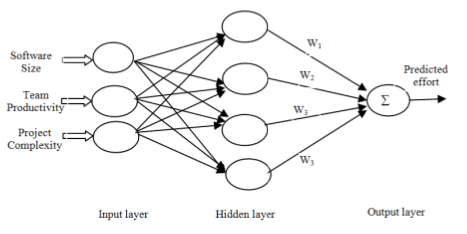
\includegraphics[natwidth=450,natheight=400,scale=.5]{Sources/Images/1.png}
\caption{Architecture of ANN}
\label{fig1}
\end{center}
\end{figure}

\section{Related Work}
\label{sec3}
\noindent{Some issues related to the UCP model have been addressed in previous work. Authors in \cite{2} and \cite{3} worked on adjustment factors, while others in highlighted the discrepancies in designing use case models. Researchers in \cite{4}, \cite{5} and \cite{6} proposed diffeerent size metrics such as Transactions, TTPoints and Paths, while others \cite{7}, \cite{8} and \cite{9} went further to extend the UCP model by providing new complexity weights or by modifying the method used to predict effort.\\
Neural network models such are and were used to predict softwa effort. Estimation using analogy such as and sort was also used for software effo prediction.\\
None of the above work deals with creating neural network models to predict software effort based on the use case points model. Moreover, our model was evaluated on industrial projects that are considered large. Another contribution of this work is to simplify the project complexity factor proposed by the UCP model by
introducing five levels of complexity levels as shown in Section \ref{sec4}.}
\section{Model's Inputs}
\label{sec4}
\noindent{The inputs of the model are software size, productivity and complexity. Software size was estimated based on the UCP model as described in Section \ref{sec2}, \ref{sub2a}.\\
The productivity factor was calculated based on Table III according to this equation:}
\begin{equation}
\small
Productivity = \sum_{i=1}^8E_i \times W_i
\end{equation}
\noindent{
Where Ei and Wi are the Environmental factors and their corresponding weights as depicted in Table \ref{table3}.
\\
The complexity of the project is an important factor in software effort prediction. Complexity can be interpreted as an item having two or more elements. There are two dimensions of complexity. These include business scope such as schedule, cost, risk and technical aspect which is the degree of difficulty in building the product. Technical complexity deals with the number of components of the product, number of technologies involved, number of interfaces and types of interfaces. The project complexity can be classified as low complexity, medium complexity or high complexity. Project complexity should be distinguished from other project characteristics such as size and uncertainty. Complex projects require more effort to develop than simple projects that have the same size. In our research, we identify the project complexity based on five levels (from Level1 to Level5). The reason behind defining five levels is to be compatible with other cost estimation models such as COCOMO where cost drivers are classified into five or six levels (such as Very Low, Low, Nominal, High, Extra High). Additionally, this classification is compatible to the project complexity classification in. Each level has its corresponding weight. The five complexity levels are defined as follows:
\begin{itemize}
\item Level1: The complexity of a project is classified as Level1 if the project team is familiar with this type of project and the team has developed similar projects in the past. The number and type of interfaces are simple. The project will be installed in normal conditions where high security or safety factors are not required. Also, Level1 projects are those of which around 20\% of their design or implementation parts are reused (came from old similar projects). The weight of the Level1 complexity is 1.
\item Level2: This is similar to level1 category with a difference that only about 10\% of these projects are reused. The weight of the Level2 complexity is 2.
\item Level3: This is the normal complexity level where projects are not said to be simple, nor complex. In this level, the technology, interface, installation conditions are normal. Furthermore, no parts of the projects had been previously
designed or implemented. The weight of the Level3 complexity is 3.
\item Level4: In this level, the project is required to be installed on a complicated topology/architecture such as distributed systems. Moreover, in this level, the number of variables and interface is large. The weight of the Level4 complexity is 4.
\item Level5: This is similar to Level4 but with additional constraints such as a special type of security or high safety factors. The weight of the Level5 complexity is 5.
\end{itemize}
\section{Regression and ANN models}
\label{sec5}
\noindent{
This section introduces the multiple regression and ANN models. Our dataset contains 240 projects. Among these projects, 70\% (168 projects) were randomly chosen to train the models and 30\% (72 projects) were used to test the model. Each of the proposed models takes 3 inputs which include software size, productivity and project complexity.
}
\subsection{Multiple Linear Regression Model}
\label{sub5a}
\noindent{The main goal of creating a multiple linear regression model from the training dataset is to compare the ANN model with the regression model. The ANN model is deemed to be valid if it outperforms the regression model. The multiple linear regression model was constructed using 168 data points. Before we apply regression on data, we applied a normality test on the variables ``Effort'' and ``Size'' and we found that ``Effort'' and ``Size'' were not normally distributed. For this purpose, ln(Effort) and ln(Size) were used instead of Effort and Size. The equation of the regression model is:
\begin{equation}
\begin{split}
\small
\ln(Effort) = 3.53+(0.88\times\ln(Size))\\
-(0.009\times Productivity)+(0.31\times Complexity).
\end{split}
\end{equation} 
\\
\noindent{To measure the accuracy of the regression model, we measured the value of the coefficient of determination R2 which is 0.88. This indicates that approximately 88 \% of the variation in Effort can be explained by the independent variables Size, Complexity and Productivity. Moreover, we measured the Analysis of Variance (ANOVA) and the model parameters. The ``p'' value of the model is 0.000 which indicates that there is a significant relationship among the variables at the 95\% confidence level. The ``p'' values of the independent variables is 0.000, this indicates that all independent variables are significant at the 95\% confidence level, and consequently the model is verified. We also measured the Variance Inflation Factor (VIF) of each independent variable to see if the multicollinearity issue (when one independent variable has a relationship with other independent variables) exists. We found that the highest VIF factor is for the variable ``Productivity'' which is 1.65. This indicates that the multicollinearity issue does not exit (VIF is less than 4). Equation (5) also shows that ``Size'' and ``Complexity'' positively correlate to ``Effort''. This means ``Productivity'' negatively correlates to ``Effort'' when software size or the complexity of the project increases, software effort would increase. On the other hand, when the team productivity of the project increases, the effort would decrease. This interpretation is compatible with the literature.}
\subsection{Artificial Neural Network}
\label{sub5b}
\noindent{Figure 1 shows the architecture of the AN used in this paper. Like the regression model, the ANN model was trained using 168 data points. One of the most important parameters of a ANN model is to determin the number of the hidden neurons. If the number is very small, the model, will not fit the data points properly. However if the number of the hidden neurons is too high, overfitting might occur. Overfitting occurs when the training error is very small but the validation/ testing error is large.\\
In our model, the conjugate gradient algorithm for training. The initial number of the hidden neurons is set to one, and then it is incremented by on until optimal results are achieved. The parameters of the model are:\\
Maximum Iterations = 10,000, Convergen Tolerance = $1.0e^{-5}$, Minimum Gradient = $1.0e^{-6}$ and Minimum Improvement Delta = $1.0e^{-6}$. To avoid overfitting the training data were held out and used for validation. If the training error is decreasing and the validation error starts to increase, the training should be stopped to a avoid overfitting. The 10-fold cross validation technique was used. At each as number of hidden neurons, the residual variance is calculated. The residual variance determin how well the model fits the dataset. The smaller the variance, the more accurate the model is. Figure 2 shows that the smallest residual variance (12.13\%) is achieved whe the number of the hidden neurons is four. DTREG software was used in developing the ANN model\\

\begin{figure}[tbp]
\begin{center}
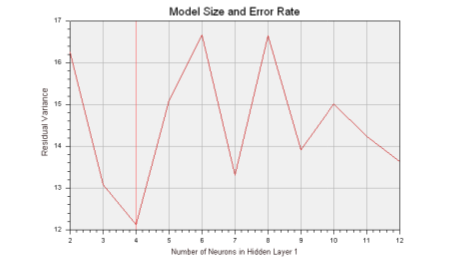
\includegraphics[natwidth=450,natheight=400,scale=.5]{Sources/Images/2.png}
\caption{Number of Hidden Neurons}
\label{fig2}
\end{center}
\end{figure}

The type of activation function used in the hidden layer is the Sigmoid (Logistic); however, the line function was used in the output layer. Figure 3 shows t actual versus the the predicted effort values.
\section{Model Evaluation and Discussion}
\label{sec6}
\noindent{This section presents the evaluatio of the proposed ANN model against the regression as well as the UCP model.\\}
\subsection{Project Dataset}
\label{sub6a}
\noindent{This research is based on software effort prediction from usecase diagrams. We have encountered many difficulties in acquiring industrial projects be
ecause revealing UML diagrams of projects is considere confidential to many companies. For this reason, we have prepared questionnaire that could help us obtain industrial data without actually having UML diagrams. In this questionnaire, we asked for example, the quantity of use cases in each project, the number of transactions of each usecase, actual software size and effo as well as the project complexity, and factors contributin to productivity. Two hundred and forty projects were collected from four main sources such that 214 are industrial projects and 26 are educational ones. The statistical profile of the project effort of the four datasets is depicted in Table \ref{table4}. S1, S2, S3 and S4 correspond to Source1, Source2 Source3 and Source4, respectively, whereas Ind and Edu correspond to Industrial and Educational, respectively.}
\vspace{0.5cm}
\begin{table}[h]
\small
\caption{Statistical Profile of datasets}
\vspace{0.5cm}
\label{table4}
\begin{tabular}{|p{1cm}|p{0.5cm}|p{0.85cm}|p{0.65cm}|p{0.65cm}|p{0.85cm}|p{0.75cm}|}
\hline
Source & \#prj & Mean & StDev & Min & Max & Skew\\
\hline
S1(Ind) & 13 & 36849.0 & 39350 & 4648 & 129353 & 1.37\\
\hline
S2(Ind) & 156 & 6225.0 & 9258 & 120 & 60826 & 3.52\\
\hline
S3(Ind) & 45 & 20573.0 & 47327 & 570 & 22480 & 3.26\\
\hline
S4(Edu) & 26 & 1689.2 & 496.6 & 850 & 2380 & -0.24\\
\hline
\end{tabular}
\end{table}
\vspace{0.5cm}

\begin{figure*}[tbp]
\begin{center}
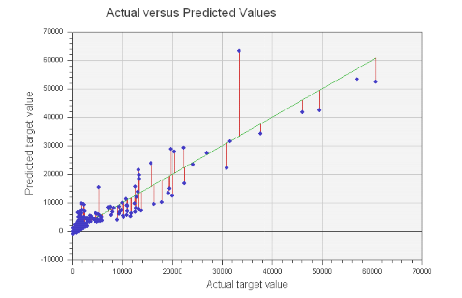
\includegraphics[natwidth=500,natheight=250]{Sources/Images/3.png}
\caption{Actual versus Predicted Effort}
\label{fig3}
\end{center}
\end{figure*}

\subsection{Model Evaluation}
\label{sub6b}
\noindent{The ANN model was evaluated using 72 data points that were not included in the training sta The criteria used are age. MMER, PRED(0.25), PRED(0.50), PRED(0.75) and PRED(1). Table V shows the values of the ANN, regression and UCP models. Figure 4 shows the interval plot at 95\% confidence level of the MMER for the three models.}
\vspace{0.5cm}
\begin{table}[h]
\small
\centering
\caption{Model Evaluation}
\vspace{0.5cm}
\label{table5}
\begin{tabular}{|p{1.65cm}|p{1cm}|p{1.35cm}|p{1cm}|}
\hline
Criteria & ANN & Regression & UCP\\
\hline
MMER & 0.49 & 0.57 & 0.99\\
\hline
PRED(0.25) & 29.16 & 29.16 & 33.33\\
\hline
PRED(0.50) & 54.16 & 63.8 & 48.61\\
\hline
PRED(0.75) & 86.11 & 87.5 & 51.38\\
\hline
PRED(1) & 90.27 & 91.6 & 61.11\\
\hline
\end{tabular}
\end{table}

\begin{figure}[tbp]
\begin{center}
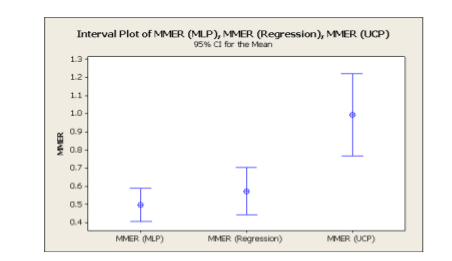
\includegraphics[natwidth=450,natheight=400,scale=.5]{Sources/Images/4.png}
\caption{Interval plot of MMER}
\label{fig4}
\end{center}
\end{figure}

\subsection{Discussion}
\label{sub6c}
\noindent{Table \ref{table5} shows that the proposed ANN model outperforms the Regression and UCP models by 8\% and 50\% respectively based on MMER. The UCP model slightly
surpasses the ANN model based on PRED(0.25). However, the ANN model gave better results in PRED(0.50), PRED(0.75) and PRED(1). Moreover, based on Figure 4, the width of the interval of the ANN model is the shortest based on MMER. This means there is no huge difference between the highest and lowest MMER values which is
good as opposed to the interval plots of other models.\\
To thoroughly evaluate the ANN model against the UCP model, a statistical test has been conducted. We applied Anderson-Darling normality test and we found that the MER of all models are not normally distributed. For this reason, we used the non-parametric Mann-Whitney test to compare the ANN with the UCP model. We found that the p-value is 0.0246. This indicates that the results are statistically significant at 95\% confidence level.}
\vspace{0.5cm}
\section{Threats to Validity}
\label{sec7}
\noindent{Threats to validity can be summarized as:\\
\begin{itemize}
\item We have encountered difficulties in collecting data especially industrial projects because companies do not reveal the UML models of their projects. For this reason, questionnaires were filled by people who work in the companies where data were collected. So we had to trust the information given to us about the datasets. For instance, an error in counting the number of the use cases or transactions will lead to an imperfection in the model's design and validation.
\item It was difficult to elicit all the environmental factors (Table \ref{table3}) from the project team. For instance, employees might incorrectly answer questions that are related to their motivation of experience.
\item Because of the lack of industrial projects, some educational projects (projects developed by students) were used. Students usually focus on the programming part when developing projects and ignore other stages in the software development life cycle, and this will underestimate the actual effort.
\end{itemize}}
\vspace{0.5cm}
%conc here
\section{Conslusions}
\label{sec8}
\noindent{This paper proposed a new feed-forward Artificial Neural Network (ANN) model to predict software effort based on the use case points model. The inputs of the proposed model are software size, productivity and project complexity. To evaluate the ANN model, a multiple linear regression model was developed that has the same inputs as the ANN model. The regression and the ANN models were trained using 168 projects and evaluated using 72 projects. The ANN model was then evaluated against the regression model as well as the Use Case Point model. Results show that the proposed ANN model outperforms the regression and UCP models based on the MMER and PRED criteria and can be used an as alternative method to predict software effort from use case diagrams.\\
Future work will focus on trying other models such as Radial Basis Function Neural Network and General Regression Neural Network.}

\begin{small}
\bibliographystyle{amsplain}
\bibliography{Sources/paper}
\end{small}
\end{document}
